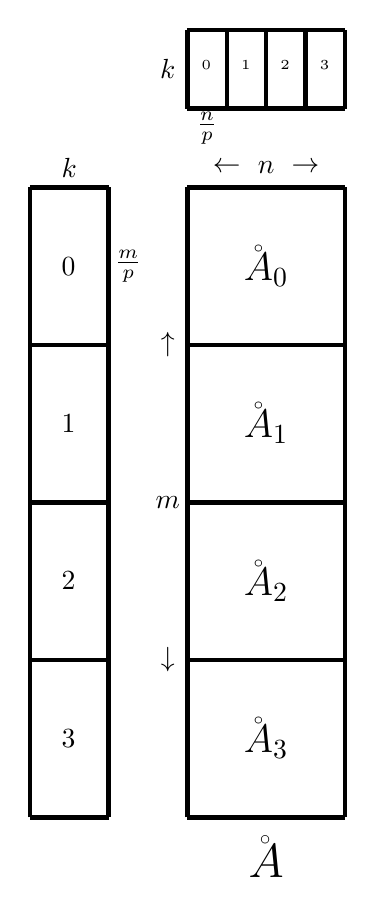
\begin{tikzpicture}

%% draw matrix distributions with scaled grids
% A
\draw[xscale=2,yscale=2,ultra thick] (0,0) grid (1,4);
% W
\draw[yscale=2,ultra thick] (-2,0) grid (-1,4);
% H
\draw[xscale=1/2,ultra thick] (0,9) grid (4,10);

%% add (sub)matrix names 
% A
\node[draw=none] at (1,-0.5) {\LARGE $\AA$};
\node[draw=none] at (1,7) {\Large $\AA_0$};
\node[draw=none] at (1,5) {\Large $\AA_1$};
\node[draw=none] at (1,3) {\Large $\AA_2$};
\node[draw=none] at (1,1) {\Large $\AA_3$};
% W
\node[draw=none] at (-1.5,-0.5) {\LARGE $\WW$};
\node[draw=none] at (-1.5,7) {\Large $\WW_0$};
\node[draw=none] at (-1.5,5) {\Large $\WW_1$};
\node[draw=none] at (-1.5,3) {\Large $\WW_2$};
\node[draw=none] at (-1.5,1) {\Large $\WW_3$};
% H
\node[draw=none] at (-1,9.5) {\LARGE $\HH$};
\node[draw=none] at (0.25,9.5) {\scriptsize $\HH^0$};
\node[draw=none] at (0.75,9.5) {\scriptsize $\HH^1$};
\node[draw=none] at (1.25,9.5) {\scriptsize $\HH^2$};
\node[draw=none] at (1.75,9.5) {\scriptsize $\HH^3$};

% label vertical dimensions
\node[draw=none] at (-0.25,9.5) {$k$};
\node[draw=none] at (-0.25,4) {$m$};
\node[draw=none] at (-0.25,6) {$\uparrow$};
\node[draw=none] at (-0.25,2) {$\downarrow$};
\node[draw=none] at (-0.75,7) {$\frac{m}{p}$};
% label horizontal dimensions
\node[draw=none] at (-1.5,8.25) {$k$};
\node[draw=none] at (1,8.25) {$n$};
\node[draw=none] at (0.5,8.25) {$\leftarrow$};
\node[draw=none] at (1.5,8.25) {$\rightarrow$};
\node[draw=none] at (0.25,8.75) {$\frac{n}{p}$};

\end{tikzpicture}
